\documentclass{article}
\usepackage[utf8]{inputenc}
\usepackage{geometry}
 \geometry{
 a4paper,
 total={170mm,257mm},
 left=20mm,
 top=20mm,
 }
 \usepackage{graphicx}
 \usepackage{subcaption}
 \usepackage{titling}
 \usepackage{float}
 \usepackage{amsmath}
\usepackage{listings}
\usepackage{color}
\usepackage{tikz}
\documentclass{article}
\usepackage{graphicx}
\usepackage{caption}
\usepackage{subcaption}
\usepackage{tikz}
\usepackage{pgfplots}
\usetikzlibrary{spy,calc}
\usepackage{hyperref}

 \title{ASSIGNMENT 2: Computer Vision 792}
\author{Madhia Shabih}
\date{August 2024}
 
 \usepackage{fancyhdr}
\fancypagestyle{plain}{%  the preset of fancyhdr 
    \fancyhf{} % clear all header and footer fields
    \fancyfoot[L]{\thedate}
    \fancyhead[L]{24397644}
    \fancyhead[R]{\theauthor}
}
\makeatletter
\def\@maketitle{%
  \newpage
  \null
  \vskip 1em%
  \begin{center}%
  \let \footnote \thanks
    {\LARGE \@title \par}%
    \vskip 1em%
    %{\large \@date}%
  \end{center}%
  \par
  \vskip 1em}
\makeatother

\usepackage{lipsum}  
\usepackage{cmbright}

\newif\ifblackandwhitecycle
\gdef\patternnumber{0}

\pgfkeys{/tikz/.cd,
    zoombox paths/.style={
        draw=orange,
        very thick
    },
    black and white/.is choice,
    black and white/.default=static,
    black and white/static/.style={ 
        draw=white,   
        zoombox paths/.append style={
            draw=white,
            postaction={
                draw=black,
                loosely dashed
            }
        }
    },
    black and white/static/.code={
        \gdef\patternnumber{1}
    },
    black and white/cycle/.code={
        \blackandwhitecycletrue
        \gdef\patternnumber{1}
    },
    black and white pattern/.is choice,
    black and white pattern/0/.style={},
    black and white pattern/1/.style={    
            draw=white,
            postaction={
                draw=black,
                dash pattern=on 2pt off 2pt
            }
    },
    black and white pattern/2/.style={    
            draw=white,
            postaction={
                draw=black,
                dash pattern=on 4pt off 4pt
            }
    },
    black and white pattern/3/.style={    
            draw=white,
            postaction={
                draw=black,
                dash pattern=on 4pt off 4pt on 1pt off 4pt
            }
    },
    black and white pattern/4/.style={    
            draw=white,
            postaction={
                draw=black,
                dash pattern=on 4pt off 2pt on 2 pt off 2pt on 2 pt off 2pt
            }
    },
    zoomboxarray inner gap/.initial=5pt,
    zoomboxarray columns/.initial=2,
    zoomboxarray rows/.initial=2,
    subfigurename/.initial={},
    figurename/.initial={zoombox},
    zoomboxarray/.style={
        execute at begin picture={
            \begin{scope}[
                spy using outlines={%
                    zoombox paths,
                    width=\imagewidth / \pgfkeysvalueof{/tikz/zoomboxarray columns} - (\pgfkeysvalueof{/tikz/zoomboxarray columns} - 1) / \pgfkeysvalueof{/tikz/zoomboxarray columns} * \pgfkeysvalueof{/tikz/zoomboxarray inner gap} -\pgflinewidth,
                    height=\imageheight / \pgfkeysvalueof{/tikz/zoomboxarray rows} - (\pgfkeysvalueof{/tikz/zoomboxarray rows} - 1) / \pgfkeysvalueof{/tikz/zoomboxarray rows} * \pgfkeysvalueof{/tikz/zoomboxarray inner gap}-\pgflinewidth,
                    magnification=3,
                    every spy on node/.style={
                        zoombox paths
                    },
                    every spy in node/.style={
                        zoombox paths
                    }
                }
            ]
        },
        execute at end picture={
            \end{scope}
            \node at (image.north) [anchor=north,inner sep=0pt] {\subcaptionbox{\label{\pgfkeysvalueof{/tikz/figurename}-image}}{\phantomimage}};
            \node at (zoomboxes container.north) [anchor=north,inner sep=0pt] {\subcaptionbox{\label{\pgfkeysvalueof{/tikz/figurename}-zoom}}{\phantomimage}};
     \gdef\patternnumber{0}
        },
        spymargin/.initial=0.5em,
        zoomboxes xshift/.initial=1,
        zoomboxes right/.code=\pgfkeys{/tikz/zoomboxes xshift=1},
        zoomboxes left/.code=\pgfkeys{/tikz/zoomboxes xshift=-1},
        zoomboxes yshift/.initial=0,
        zoomboxes above/.code={
            \pgfkeys{/tikz/zoomboxes yshift=1},
            \pgfkeys{/tikz/zoomboxes xshift=0}
        },
        zoomboxes below/.code={
            \pgfkeys{/tikz/zoomboxes yshift=-1},
            \pgfkeys{/tikz/zoomboxes xshift=0}
        },
        caption margin/.initial=4ex,
    },
    adjust caption spacing/.code={},
    image container/.style={
        inner sep=0pt,
        at=(image.north),
        anchor=north,
        adjust caption spacing
    },
    zoomboxes container/.style={
        inner sep=0pt,
        at=(image.north),
        anchor=north,
        name=zoomboxes container,
        xshift=\pgfkeysvalueof{/tikz/zoomboxes xshift}*(\imagewidth+\pgfkeysvalueof{/tikz/spymargin}),
        yshift=\pgfkeysvalueof{/tikz/zoomboxes yshift}*(\imageheight+\pgfkeysvalueof{/tikz/spymargin}+\pgfkeysvalueof{/tikz/caption margin}),
        adjust caption spacing
    },
    calculate dimensions/.code={
        \pgfpointdiff{\pgfpointanchor{image}{south west} }{\pgfpointanchor{image}{north east} }
        \pgfgetlastxy{\imagewidth}{\imageheight}
        \global\let\imagewidth=\imagewidth
        \global\let\imageheight=\imageheight
        \gdef\columncount{1}
        \gdef\rowcount{1}
        \gdef\zoomboxcount{1}
    },
    image node/.style={
        inner sep=0pt,
        name=image,
        anchor=south west,
        append after command={
            [calculate dimensions]
            node [image container,subfigurename=\pgfkeysvalueof{/tikz/figurename}-image] {\phantomimage}
            node [zoomboxes container,subfigurename=\pgfkeysvalueof{/tikz/figurename}-zoom] {\phantomimage}
        }
    },
    color code/.style={
        zoombox paths/.append style={draw=#1}
    },
    connect zoomboxes/.style={
    spy connection path={\draw[draw=none,zoombox paths] (tikzspyonnode) -- (tikzspyinnode);}
    },
    help grid code/.code={
        \begin{scope}[
                x={(image.south east)},
                y={(image.north west)},
                font=\footnotesize,
                help lines,
                overlay
            ]
            \foreach \x in {0,1,...,9} { 
                \draw(\x/10,0) -- (\x/10,1);
                \node [anchor=north] at (\x/10,0) {0.\x};
            }
            \foreach \y in {0,1,...,9} {
                \draw(0,\y/10) -- (1,\y/10);                        \node [anchor=east] at (0,\y/10) {0.\y};
            }
        \end{scope}    
    },
    help grid/.style={
        append after command={
            [help grid code]
        }
    },
}

\newcommand\phantomimage{%
    \phantom{%
        \rule{\imagewidth}{\imageheight}%
    }%
}
\newcommand\zoombox[2][]{
    \begin{scope}[zoombox paths]
        \pgfmathsetmacro\xpos{
            (\columncount-1)*(\imagewidth / \pgfkeysvalueof{/tikz/zoomboxarray columns} + \pgfkeysvalueof{/tikz/zoomboxarray inner gap} / \pgfkeysvalueof{/tikz/zoomboxarray columns} ) + \pgflinewidth
        }
        \pgfmathsetmacro\ypos{
            (\rowcount-1)*( \imageheight / \pgfkeysvalueof{/tikz/zoomboxarray rows} + \pgfkeysvalueof{/tikz/zoomboxarray inner gap} / \pgfkeysvalueof{/tikz/zoomboxarray rows} ) + 0.5*\pgflinewidth
        }
        \edef\dospy{\noexpand\spy [
            #1,
            zoombox paths/.append style={
                black and white pattern=\patternnumber
            },
            every spy on node/.append style={#1},
            x=\imagewidth,
            y=\imageheight
        ] on (#2) in node [anchor=north west] at ($(zoomboxes container.north west)+(\xpos pt,-\ypos pt)$);}
        \dospy
        \pgfmathtruncatemacro\pgfmathresult{ifthenelse(\columncount==\pgfkeysvalueof{/tikz/zoomboxarray columns},\rowcount+1,\rowcount)}
        \global\let\rowcount=\pgfmathresult
        \pgfmathtruncatemacro\pgfmathresult{ifthenelse(\columncount==\pgfkeysvalueof{/tikz/zoomboxarray columns},1,\columncount+1)}
        \global\let\columncount=\pgfmathresult
        \ifblackandwhitecycle
            \pgfmathtruncatemacro{\newpatternnumber}{\patternnumber+1}
            \global\edef\patternnumber{\newpatternnumber}
        \fi
    \end{scope}
}

\begin{document}
\maketitle
\section{Question 1}

\texttt{q1.py} performs a series of projective transformations (specifically similarity transformations) on an image. The key steps and functionality are as follows:

\begin{itemize}
    \item The necessary libraries are imported, including \texttt{numpy} for numerical operations, \texttt{applyhomography} for applying homography transformations, \texttt{math} for mathematical operations, and \texttt{PIL} (Python Imaging Library) for image processing.
    \item The image \texttt{afghanGirl.jpg} is loaded and converted to a NumPy array.
    \item Three lists of scaling factors ($s$), and translation values ($tx$ and $ty$) are defined.
    \item The code iterates over all combinations of these values to create a series of similarity transformation matrices using the following formula:
    \[
    H = \begin{bmatrix}
    s \cos(\pi/4) & -s \sin(\pi/4) & tx \\
    s \sin(\pi/4) & s \cos(\pi/4) & ty \\
    0 & 0 & 1
    \end{bmatrix}
    \]
    \item For each transformation matrix $H$, the \texttt{applyhomography} function is applied to the image to produce a transformed image.
    \item The transformed images are saved with filenames indicating the parameters used in the transformation, such as \texttt{output/similar\_s\_tx\_ty.jpg}.
\end{itemize}

\begin{figure}[H]
    \centering
    \begin{subfigure}{.3\textwidth}
        \centering
        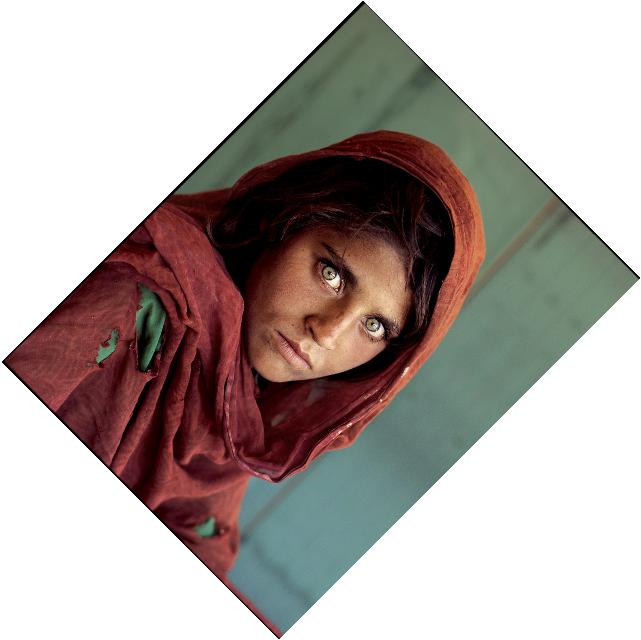
\includegraphics[scale=0.04]{q1/output/similar_0.5_0.5_2.jpg}
        \subcaption{x-translation value of 0.5}
    \end{subfigure}
    \begin{subfigure}{.3\textwidth}
        \centering
        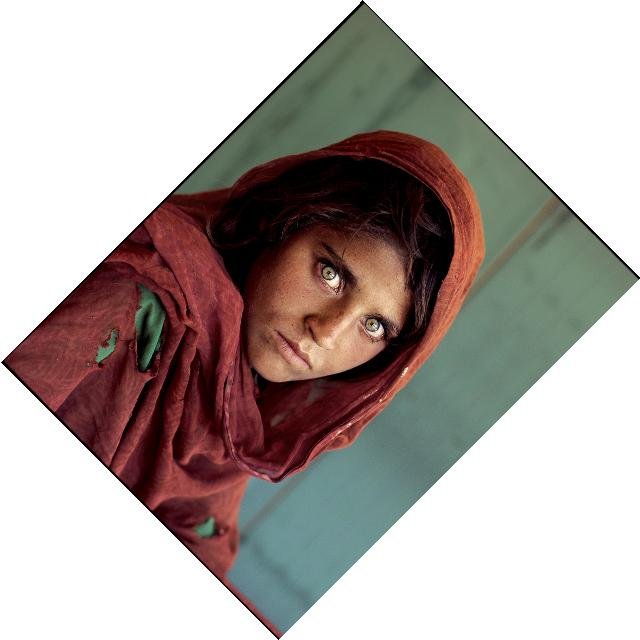
\includegraphics[scale=0.04]{q1/output/similar_0.5_1_2.jpg}
        \subcaption{x-translation value of 1}
    \end{subfigure}
    \begin{subfigure}{.3\textwidth}
        \centering
        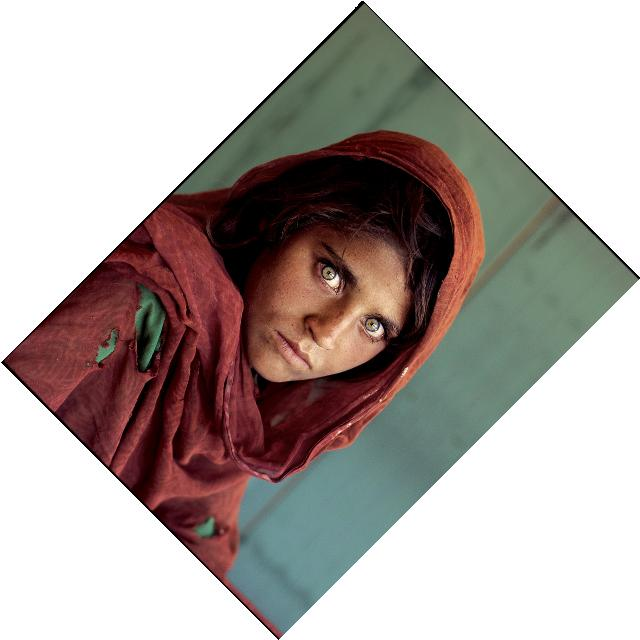
\includegraphics[scale=0.04]{q1/output/similar_0.5_2_2.jpg}
        \subcaption{x-translation value of 2}
    \end{subfigure}
    \caption{Scaling factor of 0.5 and y-translation value of 2}
\end{figure}

\begin{figure}[H]
    \centering
    \begin{subfigure}{.3\textwidth}
        \centering
        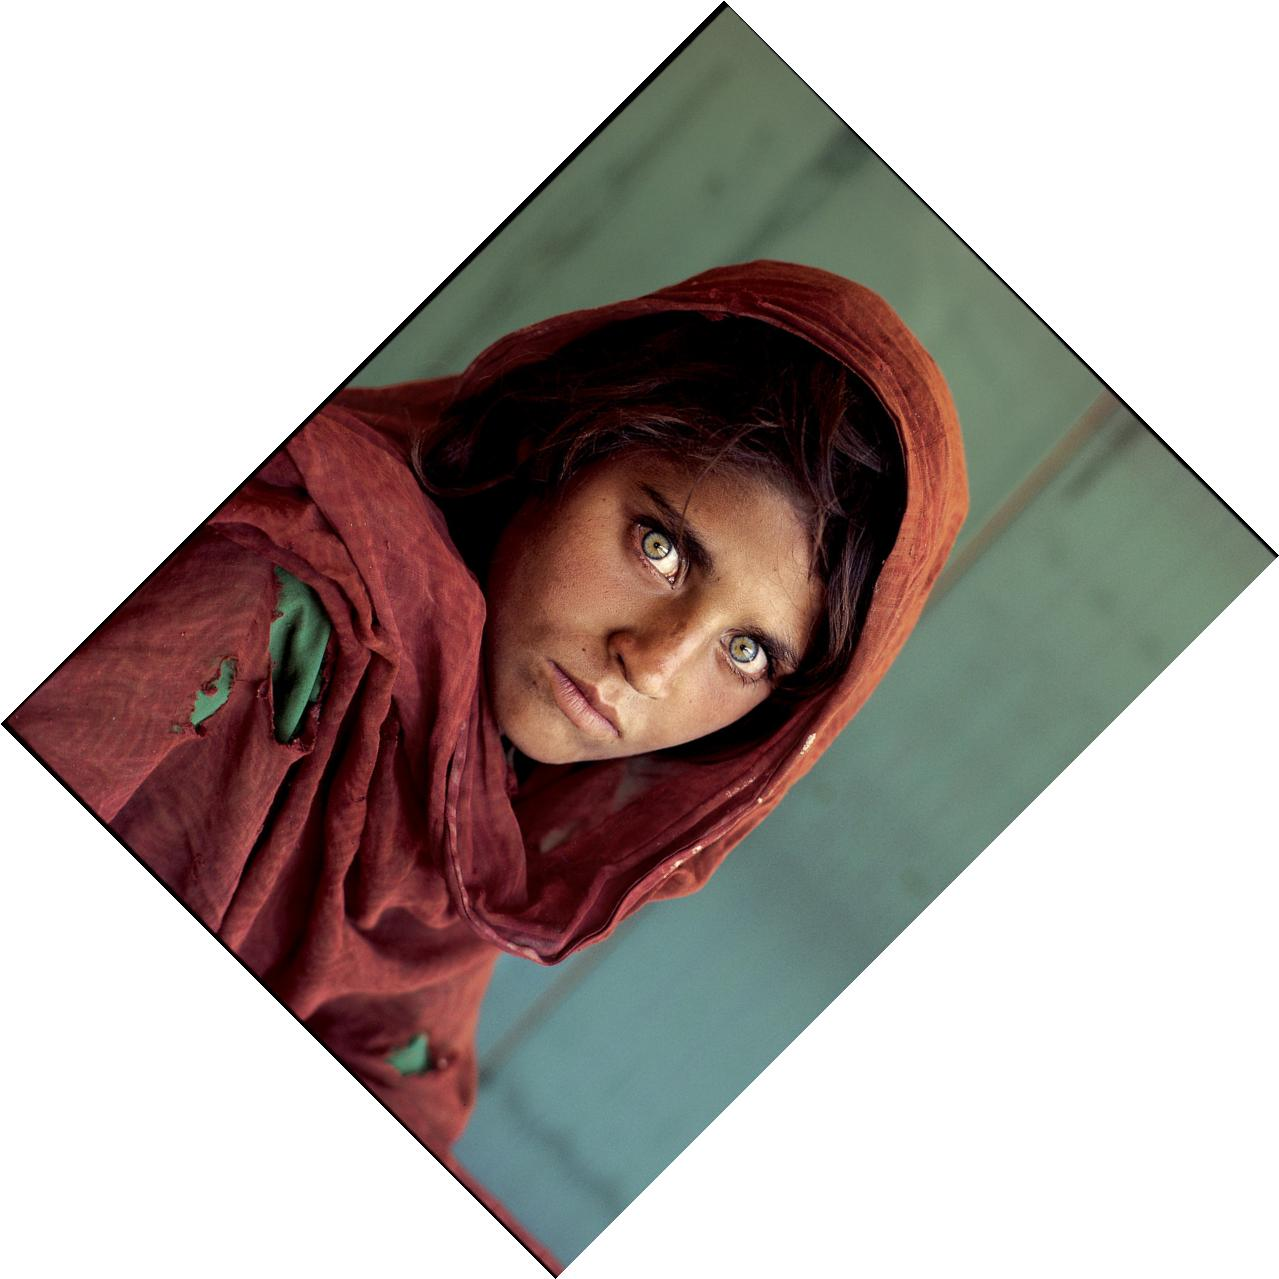
\includegraphics[scale=0.04]{q1/output/similar_1_0.5_2.jpg}
        \subcaption{x-translation value of 0.5}
    \end{subfigure}
    \begin{subfigure}{.3\textwidth}
        \centering
        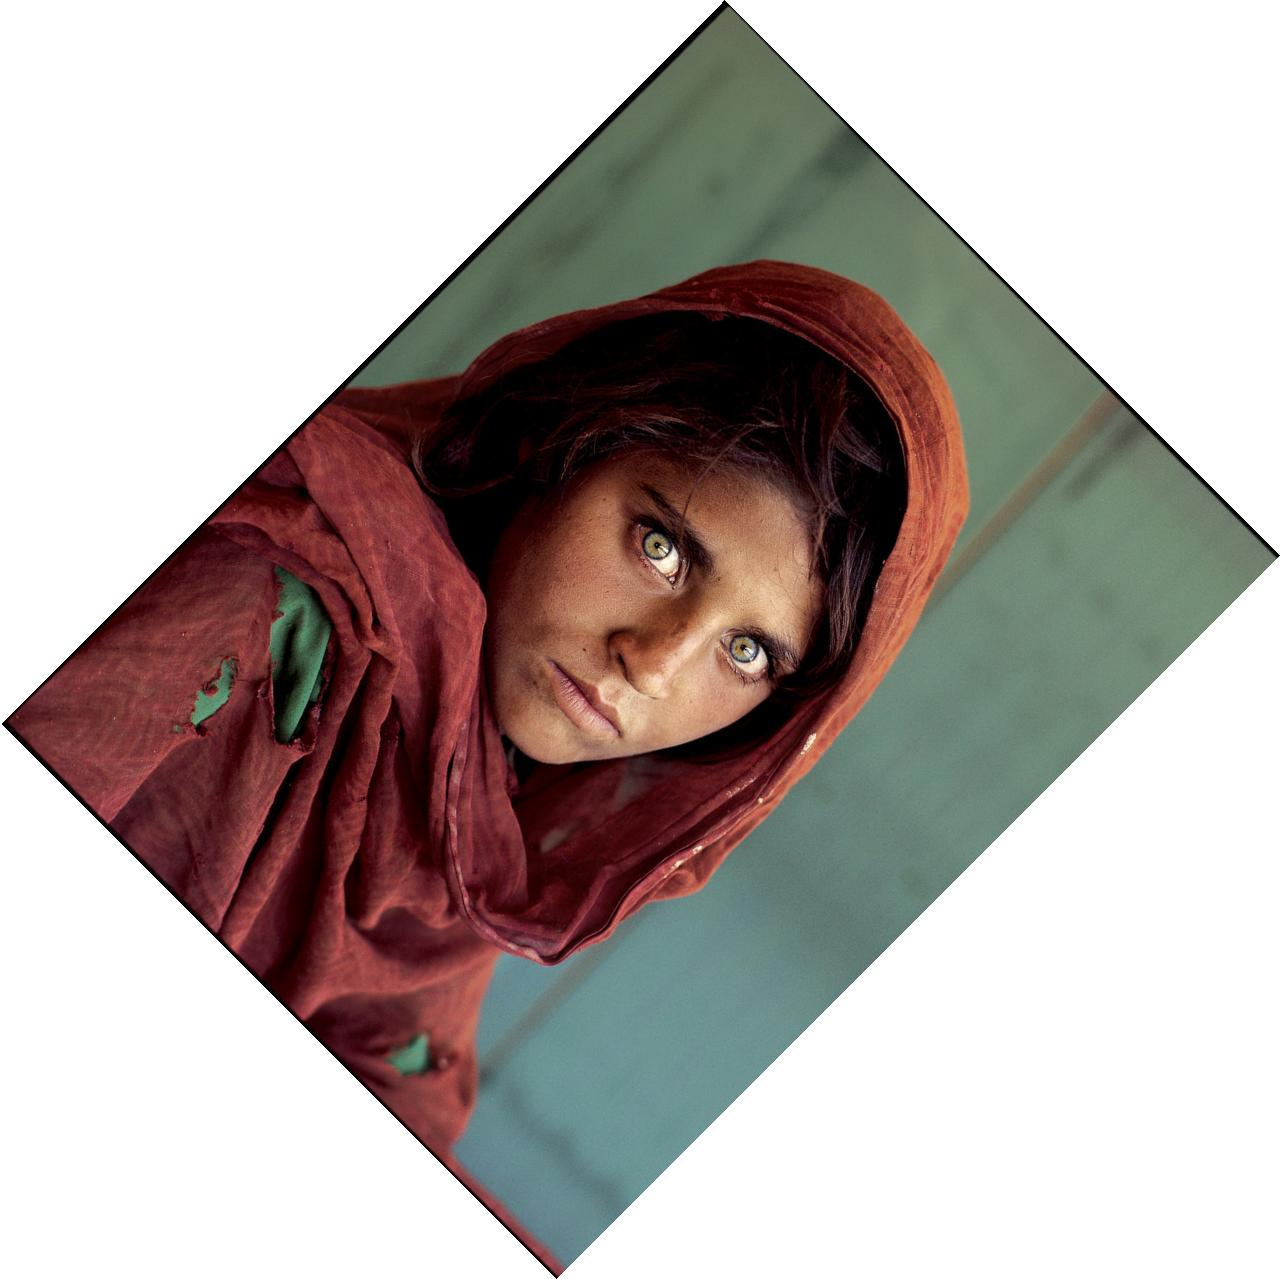
\includegraphics[scale=0.04]{q1/output/similar_1_1_2.jpg}
        \subcaption{x-translation value of 1}
    \end{subfigure}
    \begin{subfigure}{.3\textwidth}
        \centering
        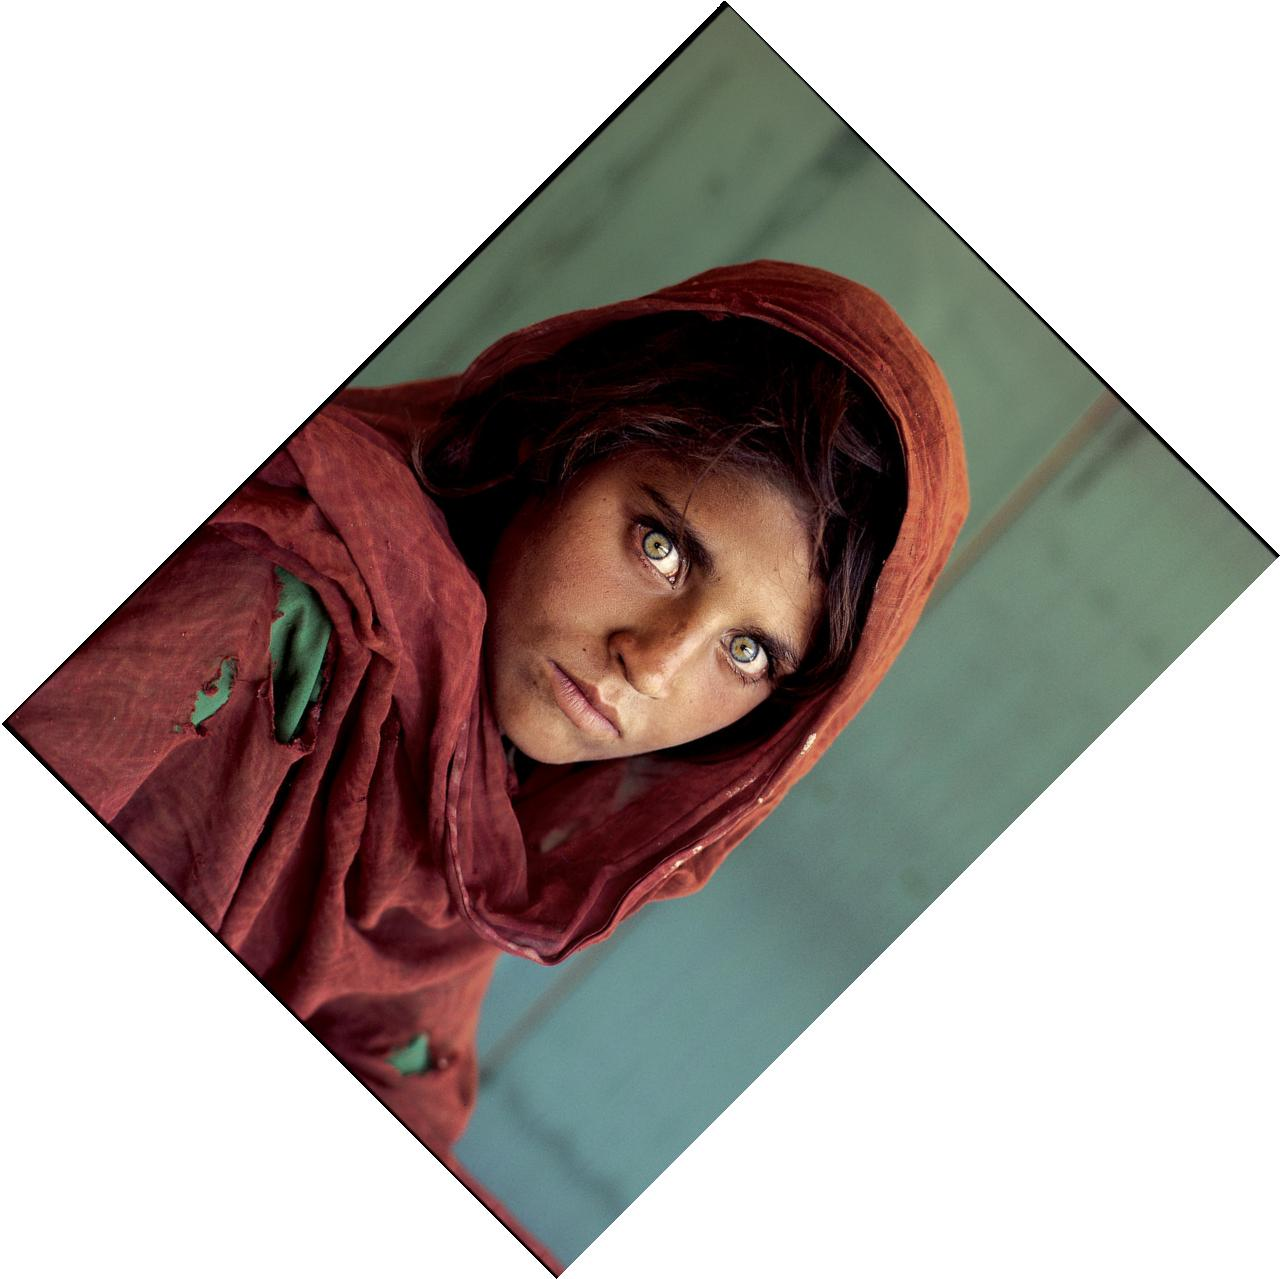
\includegraphics[scale=0.04]{q1/output/similar_1_2_2.jpg}
        \subcaption{x-translation value of 2}
    \end{subfigure}
    \caption{Scaling factor of 1 and y-translation value of 2}
\end{figure}

\begin{figure}[H]
    \centering
    \begin{subfigure}{.3\textwidth}
        \centering
        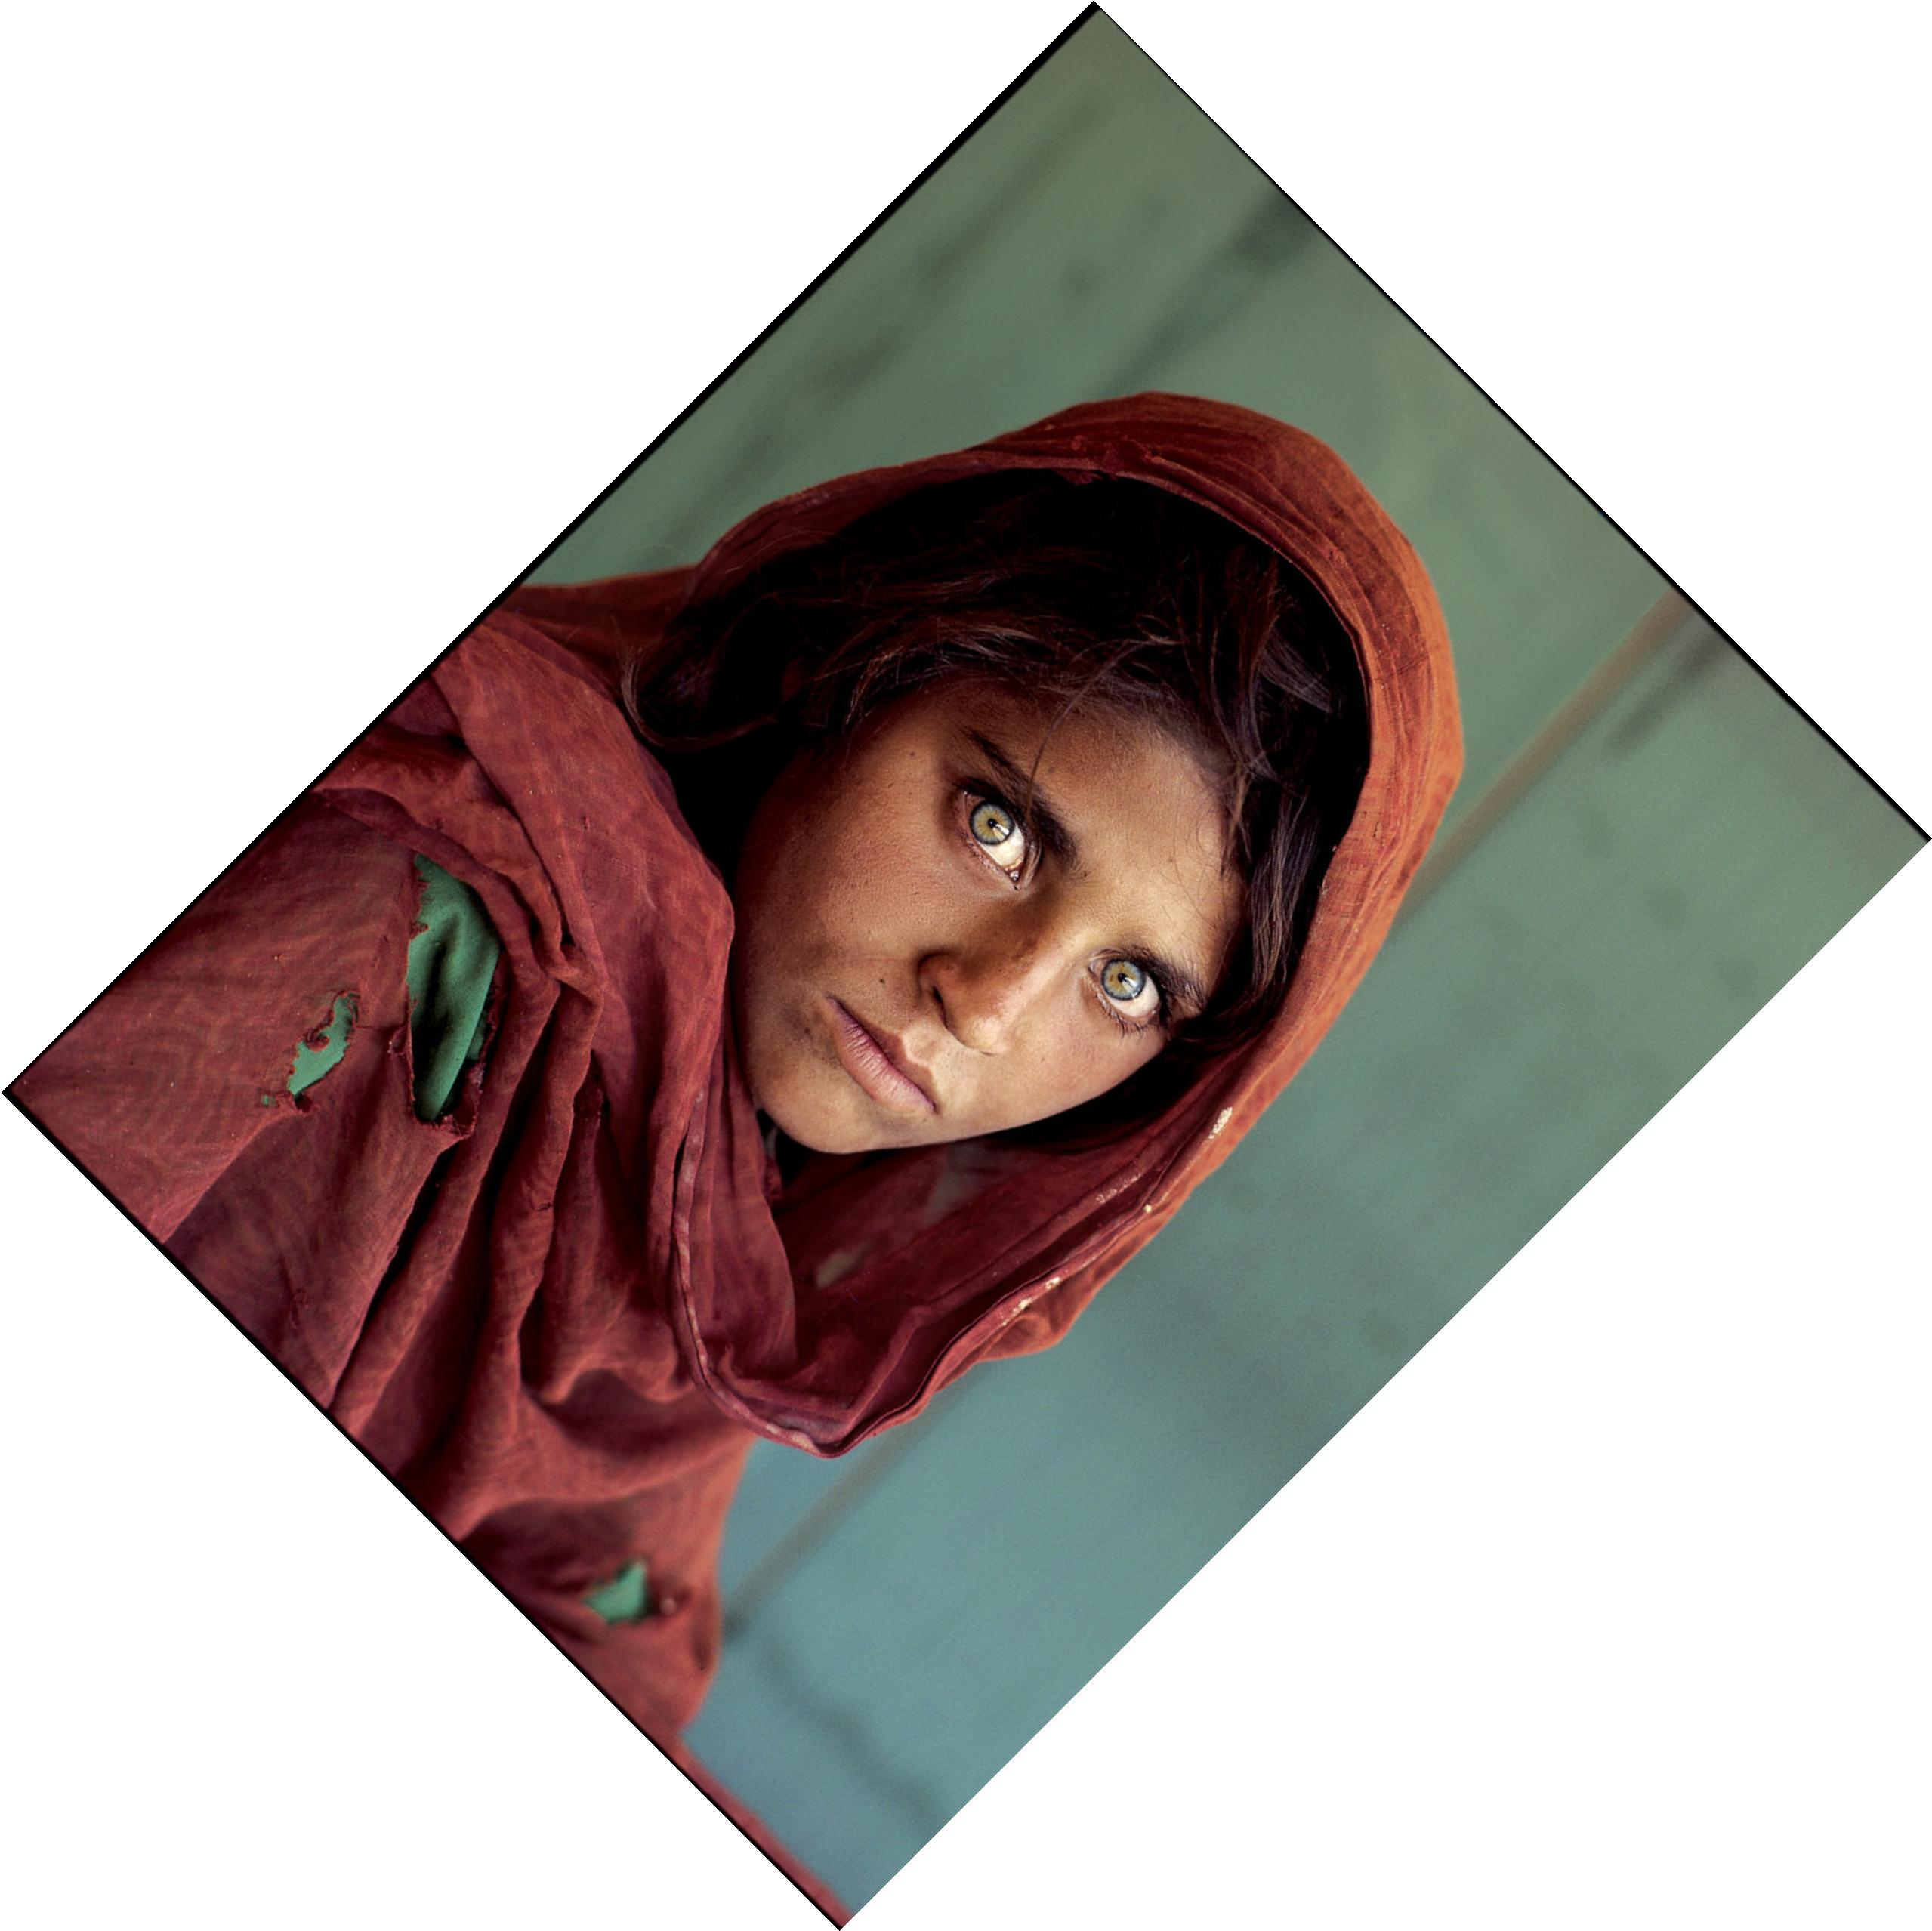
\includegraphics[scale=0.04]{q1/output/similar_2_0.5_2.jpg}
        \subcaption{x-translation value of 0.5}
    \end{subfigure}
    \begin{subfigure}{.3\textwidth}
        \centering
        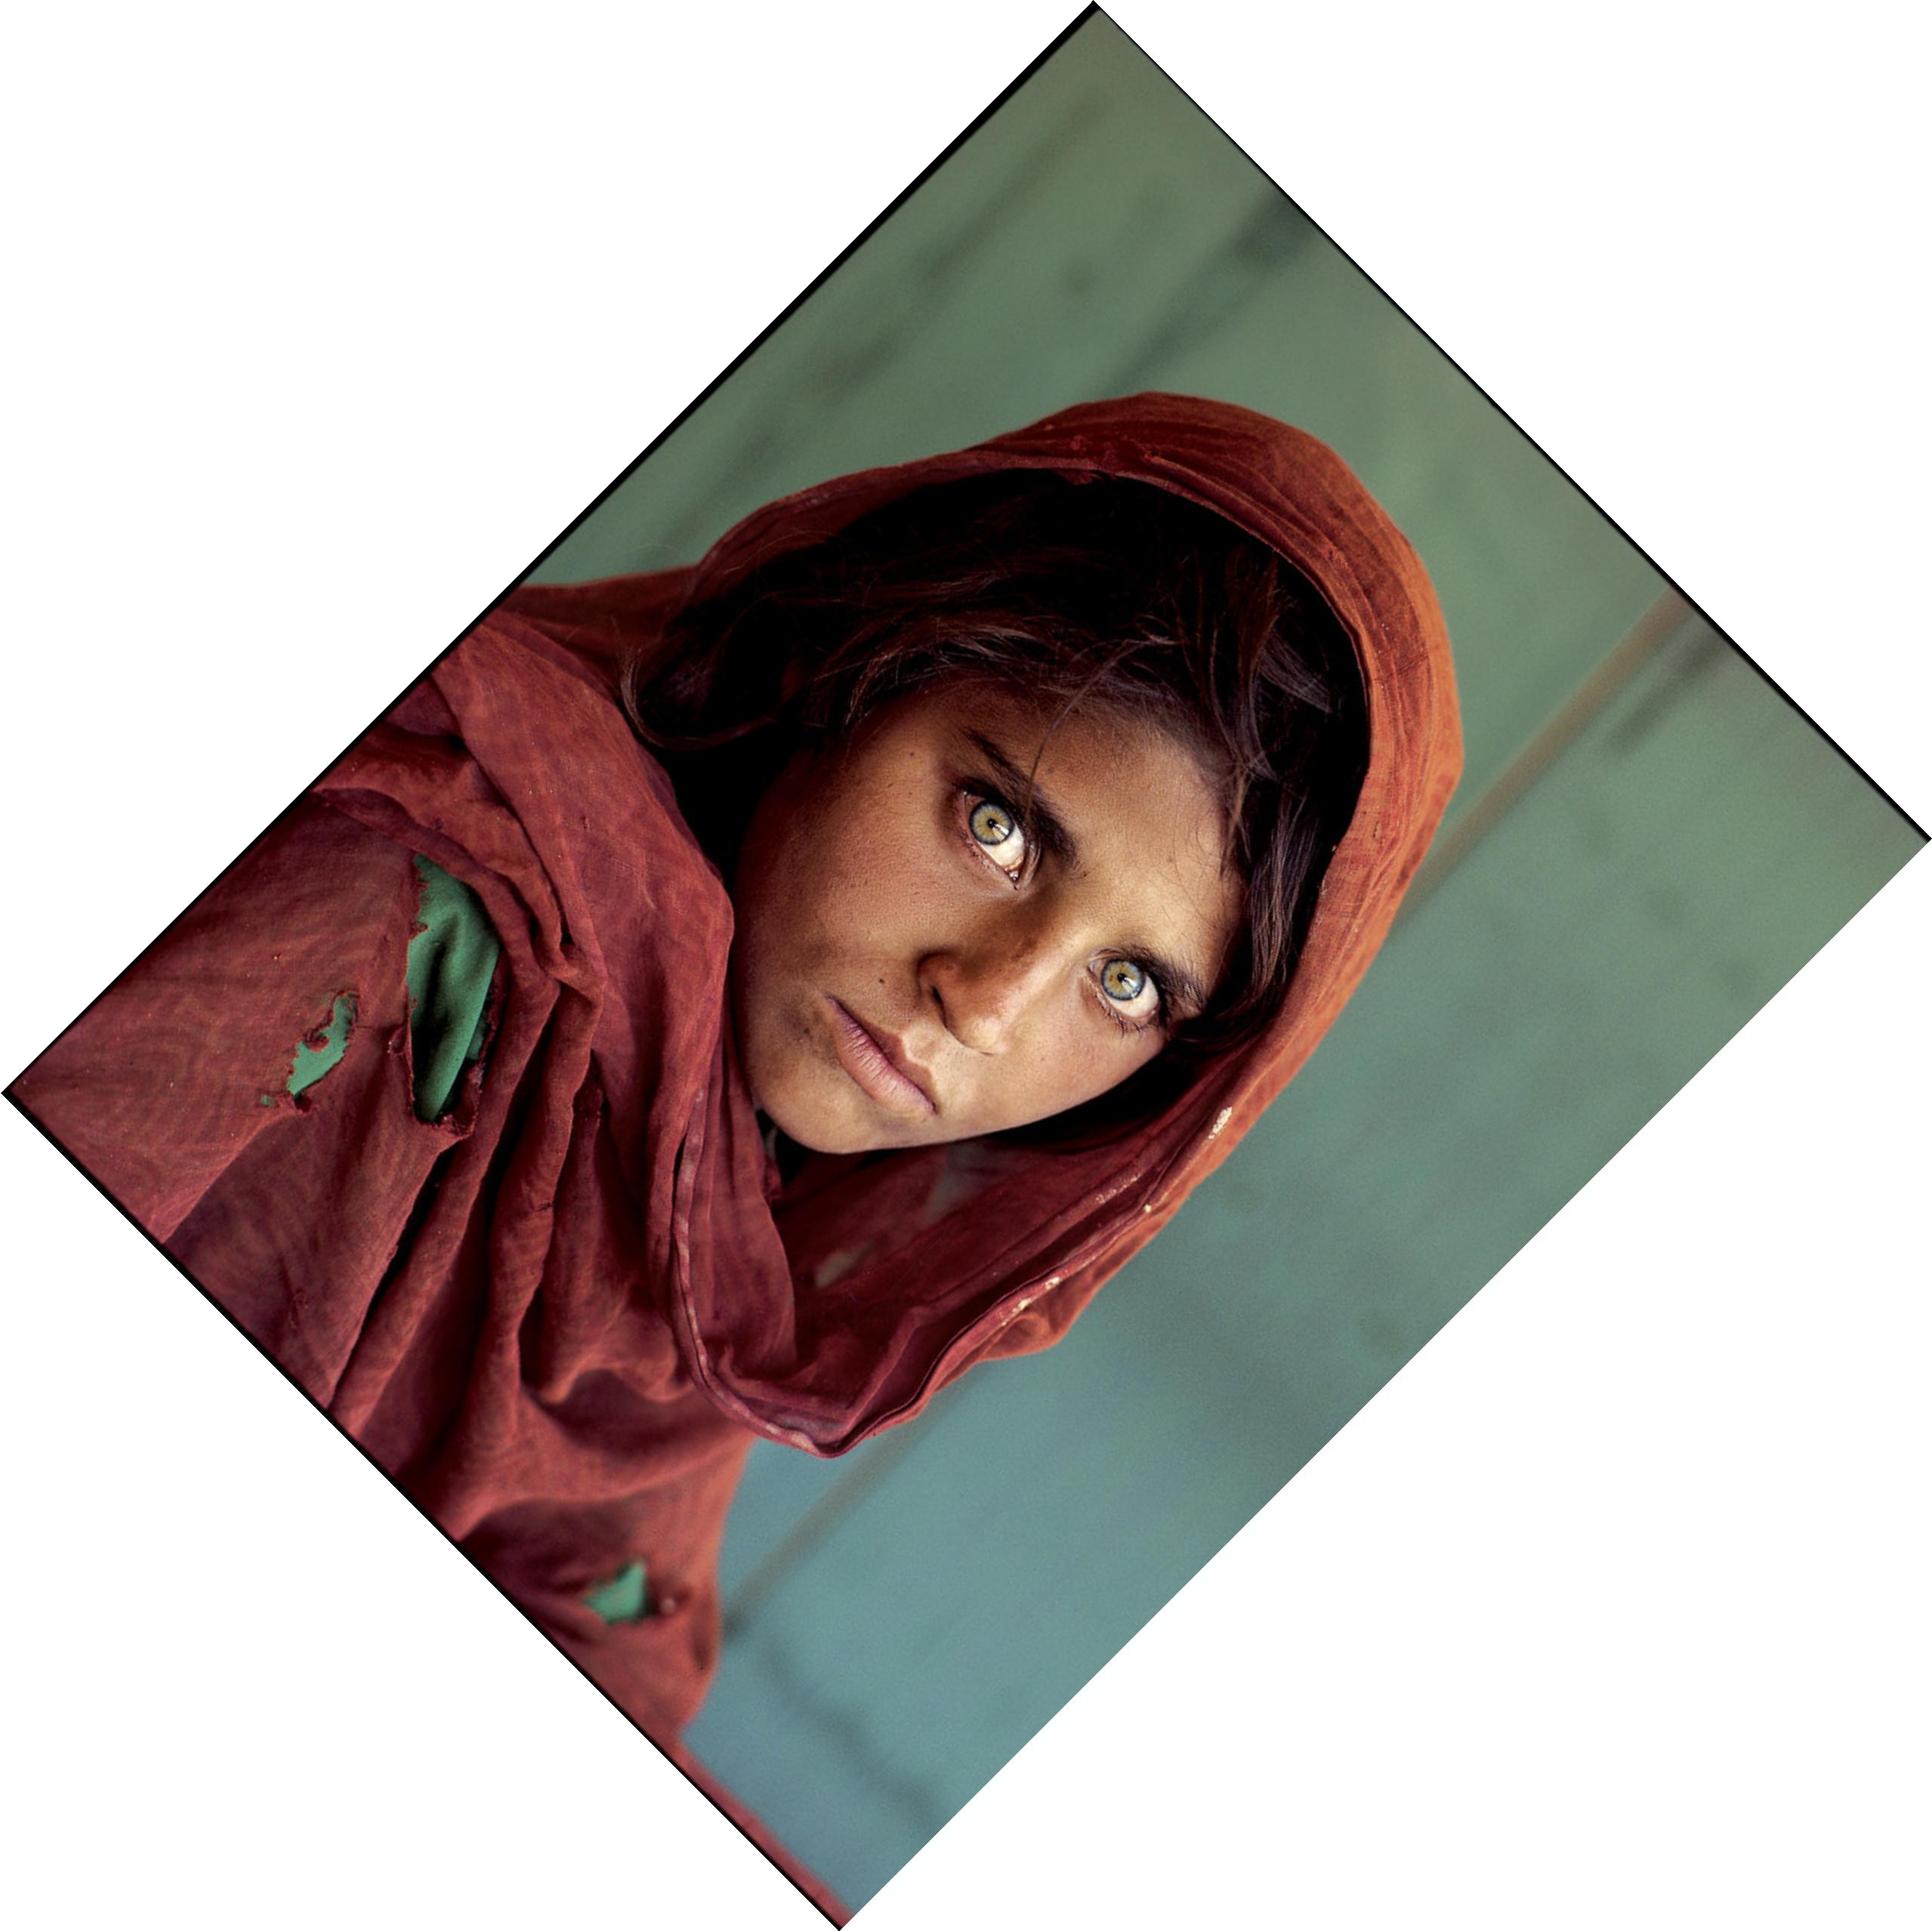
\includegraphics[scale=0.04]{q1/output/similar_2_1_2.jpg}
        \subcaption{x-translation value of 1}
    \end{subfigure}
    \begin{subfigure}{.3\textwidth}
        \centering
        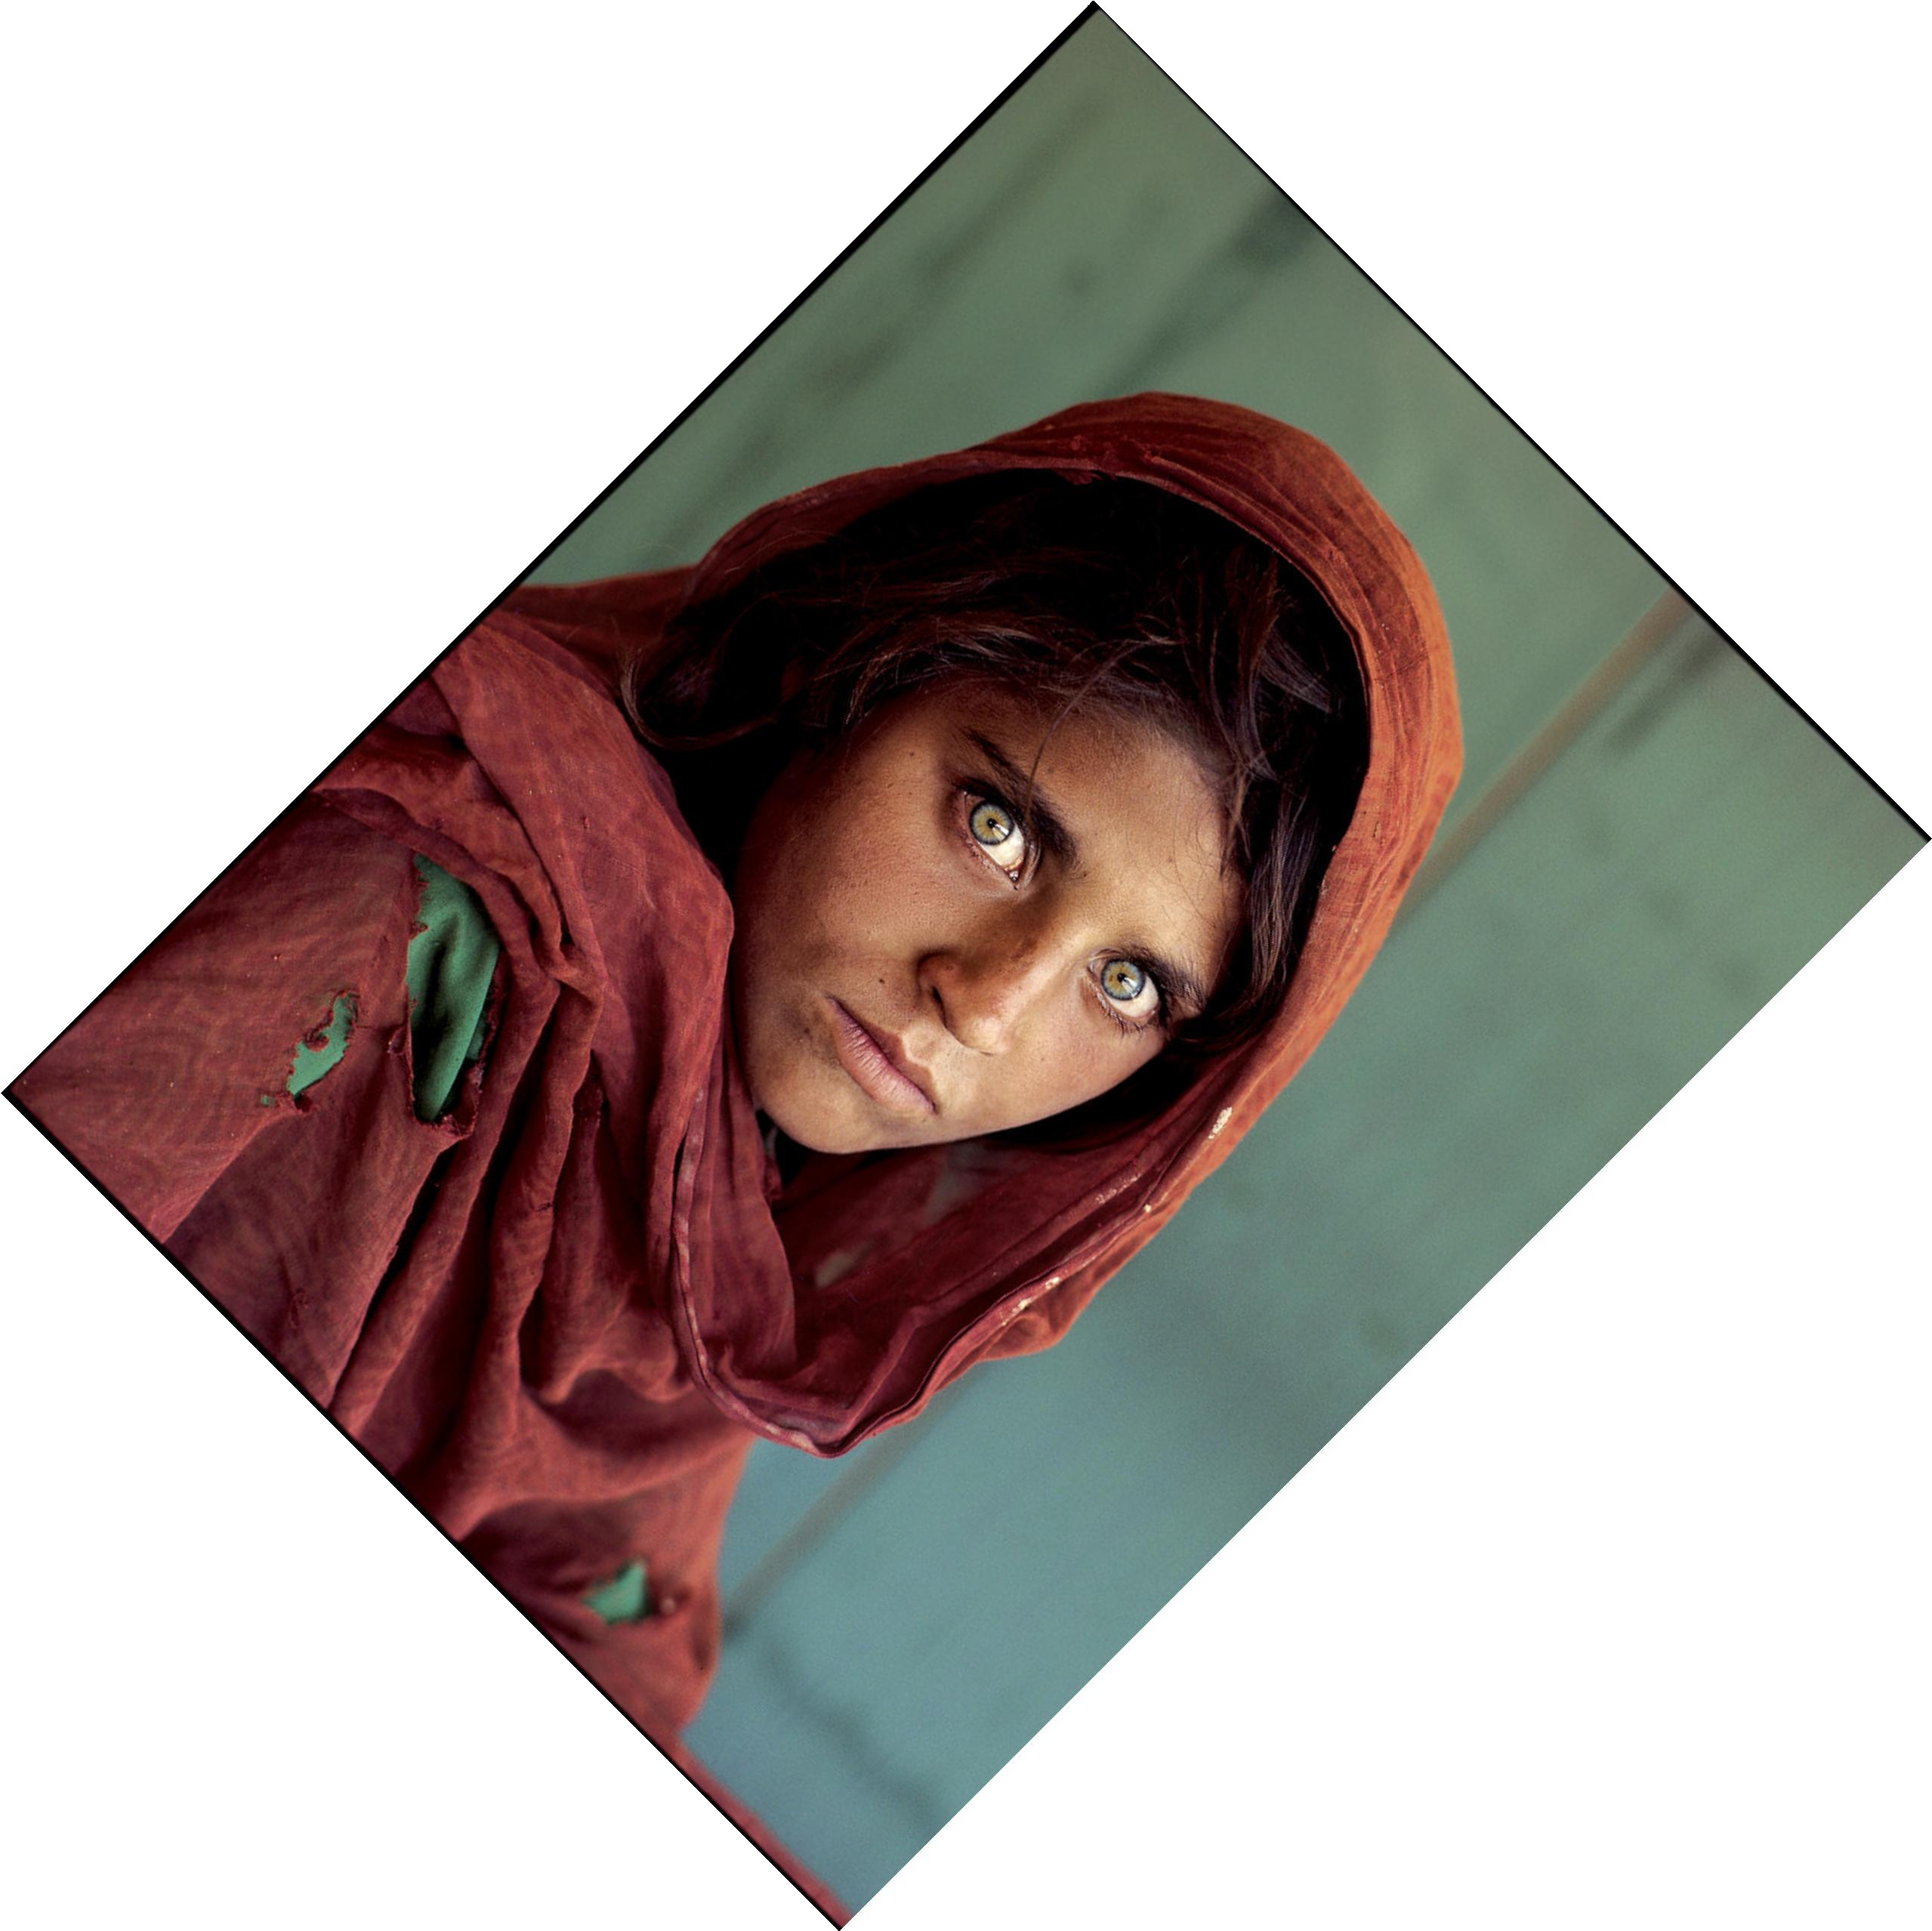
\includegraphics[scale=0.04]{q1/output/similar_2_2_2.jpg}
        \subcaption{x-translation value of 2}
    \end{subfigure}
    \caption{Scaling factor of 2 and y-translation value of 2}
\end{figure}

\subsection{Interpretation}
The \texttt{applyhomography.py} function is designed to compensate for the shift in the output image's origin. The code transforms the four corners of the input image using the homography matrix H. 
It then finds the minimum and maximum x and y coordinates. The size of the output image is then set to encompass all these points. 
This is why we do not see an impact of the translations on the image. 

%%%%%%%%%%%%%%%%%%%%
\section{Question 2}
\texttt{q2.py} performs a homography transformation on an image and pastes it onto another image. Below is a detailed breakdown:

\begin{itemize}
    \item \textbf{Libraries Used:} The code utilizes \texttt{numpy}, \texttt{numpy.linalg}, and \texttt{PIL.Image} for numerical operations, linear algebra, and image processing, respectively.
    
    \item \textbf{apply\_homography Function:} 
    \begin{itemize}
        \item This function takes an image \texttt{A} and a homography matrix \texttt{H}, then applies the homography transformation.
        \item The image's corners are transformed using the homography matrix to determine the size of the transformed output.
        \item The inverse homography matrix is used to map each pixel in the output image back to the original image for interpolation.
        \item Pixels are interpolated using bilinear interpolation, and pixels outside the transformed region are set to white.
    \end{itemize}
    
    \item \textbf{find\_homography Function:} 
    \begin{itemize}
        \item This function computes the homography matrix \texttt{H} using four pairs of corresponding points from the source and destination images.
        \item It sets up a system of linear equations and solves it using Singular Value Decomposition (SVD) to find the homography matrix.
    \end{itemize}
    
    \item \textbf{Image Processing:}
    \begin{itemize}
        \item The code loads a poster image and a building image.
        \item It defines source points from the poster and corresponding destination points on the building image.
        \item The homography matrix is calculated using these points.
        \item The poster is transformed using the homography matrix, and the resulting image is then pasted onto the building image.
        \item A mask is created to ensure only non-white pixels of the transformed image are pasted.
        \item The final composite image is saved as \texttt{output.jpg}, and the transformed poster is saved as \texttt{transform.jpg}.
    \end{itemize}
\end{itemize}

\begin{figure}[H]
    \centering
    \begin{subfigure}{.3\textwidth}
        \centering
        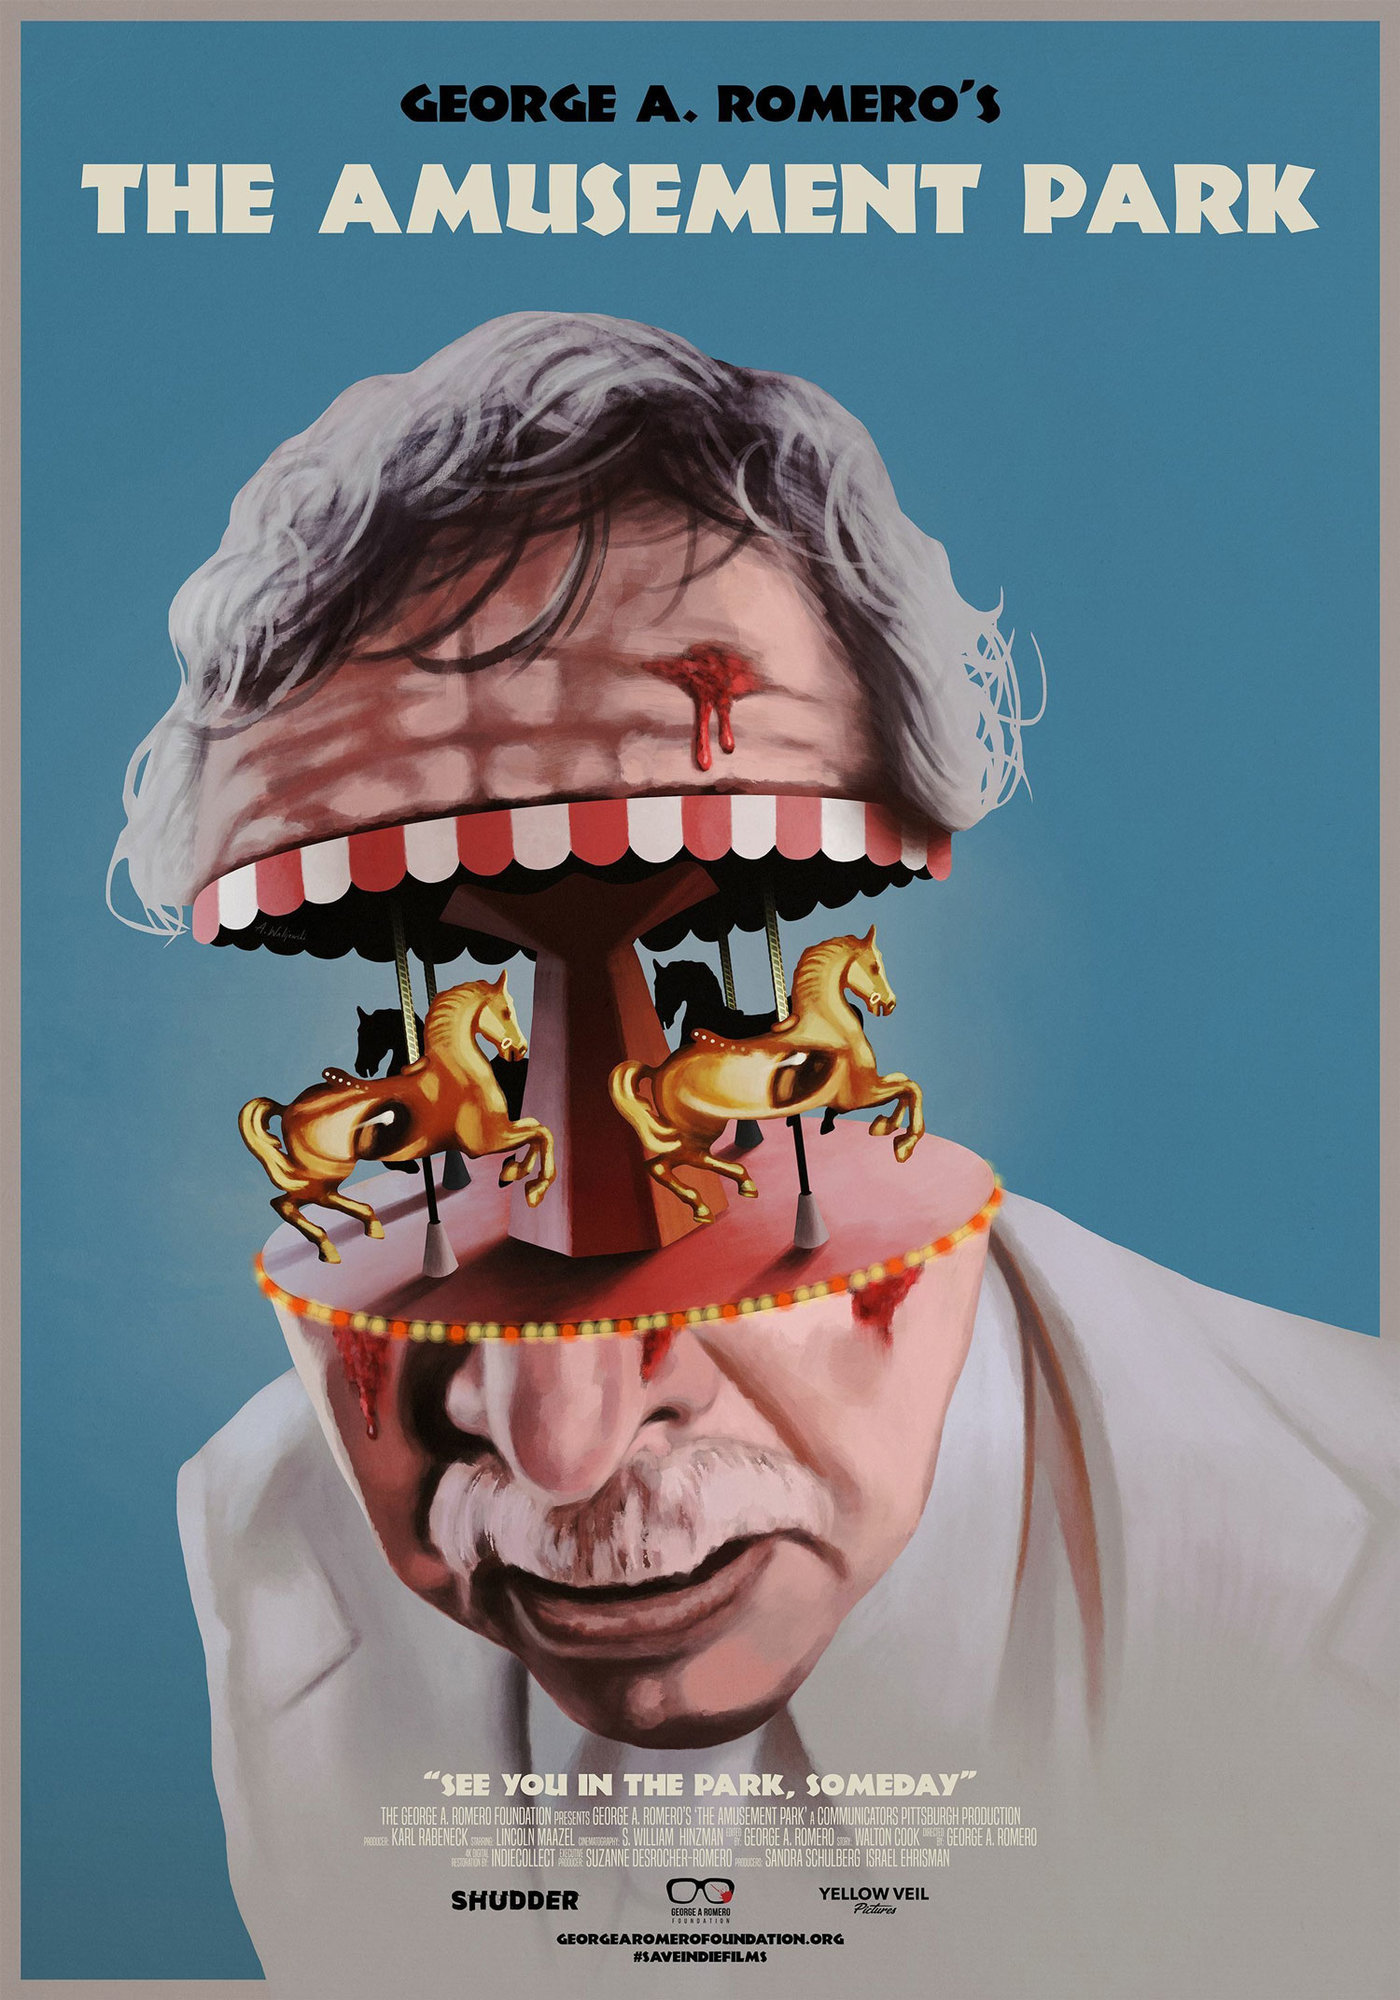
\includegraphics[scale=0.1]{q2/amuse.jpg}
        \subcaption{Original Movie Poster}
    \end{subfigure}
    \begin{subfigure}{.3\textwidth}
        \centering
        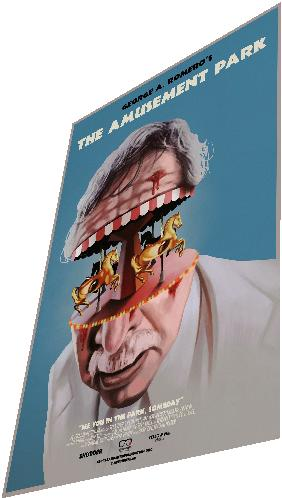
\includegraphics[scale=0.3]{q2/output/transform.jpg}
        \subcaption{Transformed Movie Poster}  
        \label{fig 1}
    \end{subfigure}
    \begin{subfigure}{.3\textwidth}
        \centering
        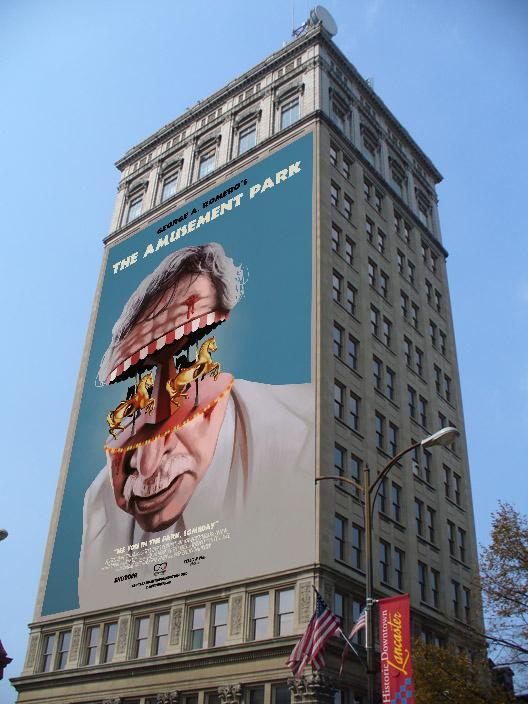
\includegraphics[scale=0.3]{q2/output/output.jpg}
        \caption{Building with Movie Poster}  
        \label{fig 2}
    \end{subfigure}
\end{figure}

\subsection{Interpretation}
%The transformed poster image will contain parts with no
%image data that we want to ignore, and the image origin
%may shift (why?). Explain how you addressed these two
%issues.
The transformed poster image contains a white region where there is no image data because the transformation maps some parts of the image
to areas that fall outside the original image bounds. To handle this, I created a mask: When pasting the transformed poster onto the building, 
the mask ensures that only the parts of the poster with actual content are pasted.

After applying the transformation, the origin of the poster shifts to a different position. This happens because the transformation can move the 
image in ways that push it outside the original image boundries. I compensate for this by calculating \texttt{minx} and \texttt{miny}. These
represent how much the image has shifted in the negative direction from the origin \texttt{(0,0)}. In this case, the minimum x and minimum y co-ordinates
shift by 35 and 124 units respectively. This offset ensures that the transformed poster aligns correctly with the intended location on the building image.

% Also, if we follow the interpolation procedure in the given code that applies homographies to images, it
% turns out that our input (untransformed) poster image should be more-or-less similar in size to the desired
% output (the transformed image). If the input is much larger, we get undesired “aliasing” artefacts in the
% output. Experiment with this idea, and include in your report a short explanation of the issue of aliasing
% in image interpolation.

The original image is of size 1400 x 2000 and the building image is of size 528 x 704. 
\subsubsection{Case 1 : Large Input Image}
As one can observe in \ref{fig 1} and \ref{fig 2}. 
As one can observe, there are aliasing artifacts such as jagged edges and loss of fine detail. The downscaling process during the transformation 
fails to adequately capture the high frequency content. 

\subsubsection{Case 2 : Input Image of Same Size}
The input image was changed to 528 x 704 to resemble the size of the output image.
As one can observe, the image suffers from minimal aliasing. 

\subsubsection{Case 3 : Small Input Image}
The input image was now 250 x 350. The output poster is more blurred, but there are not as much aliasing 
artifacts as there were when the image was larger.

\begin{figure}[H]\centering
    \begin{tikzpicture}[
        zoomboxarray,black and white=cycle,
    ]
        \node [image node] { 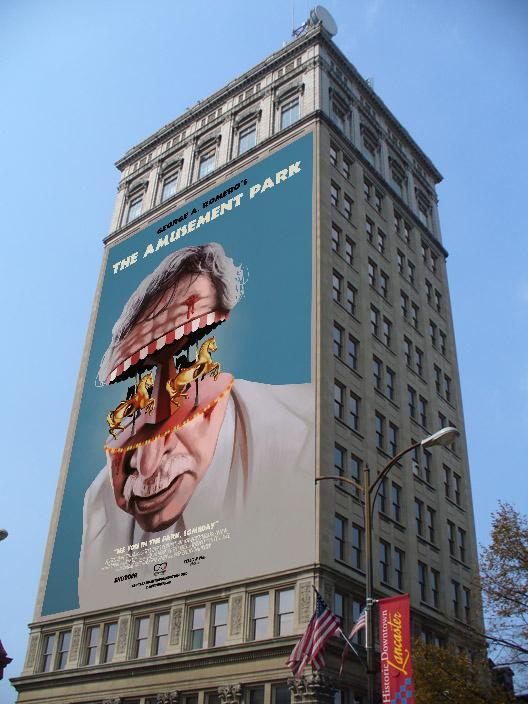
\includegraphics[width=0.45\textwidth]{q2/output/output.jpg} };
        \zoombox{0.5,0.5}
        \zoombox[color code=red,magnification=6]{0.3,0.3}
        \zoombox{0.42,0.45}
        \zoombox[magnification=5]{0.4,0.7}
    \end{tikzpicture}
    \caption{Building with 1400x2000 Movie Poster}
    \end{figure}
\begin{figure}[H]\centering
    \begin{tikzpicture}[
        zoomboxarray,black and white=cycle,
    ]
        \node [image node] { 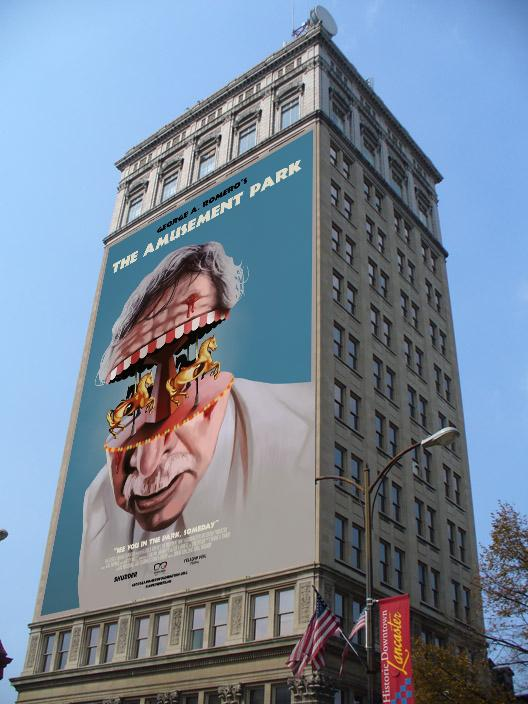
\includegraphics[width=0.45\textwidth]{q2/output/output_same.jpg} };
        \zoombox{0.5,0.5}
        \zoombox[color code=red,magnification=6]{0.3,0.3}
        \zoombox{0.42,0.45}
        \zoombox[magnification=5]{0.4,0.7}
    \end{tikzpicture}
    \caption{Building with 528x704 Movie Poster}
    \end{figure}    
\begin{figure}[H]\centering
    \begin{tikzpicture}[
        zoomboxarray,black and white=cycle,
    ]
        \node [image node] { 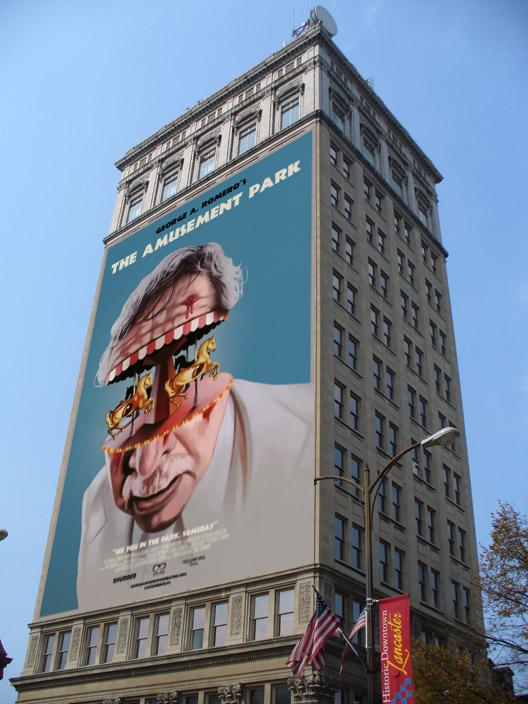
\includegraphics[width=0.45\textwidth]{q2/output/output_small.jpg} };
        \zoombox{0.5,0.5}
        \zoombox[color code=red,magnification=6]{0.3,0.3}
        \zoombox{0.42,0.45}
        \zoombox[magnification=5]{0.4,0.7}
    \end{tikzpicture}
    \caption{Building with 250x250 Movie Poster}
    \end{figure}
    

%%%%%%%%%%%%%%%%%%%%
\section{Question 3}
\begin{figure}[H]
    \centering
    \begin{subfigure}{.3\textwidth}
        \centering
        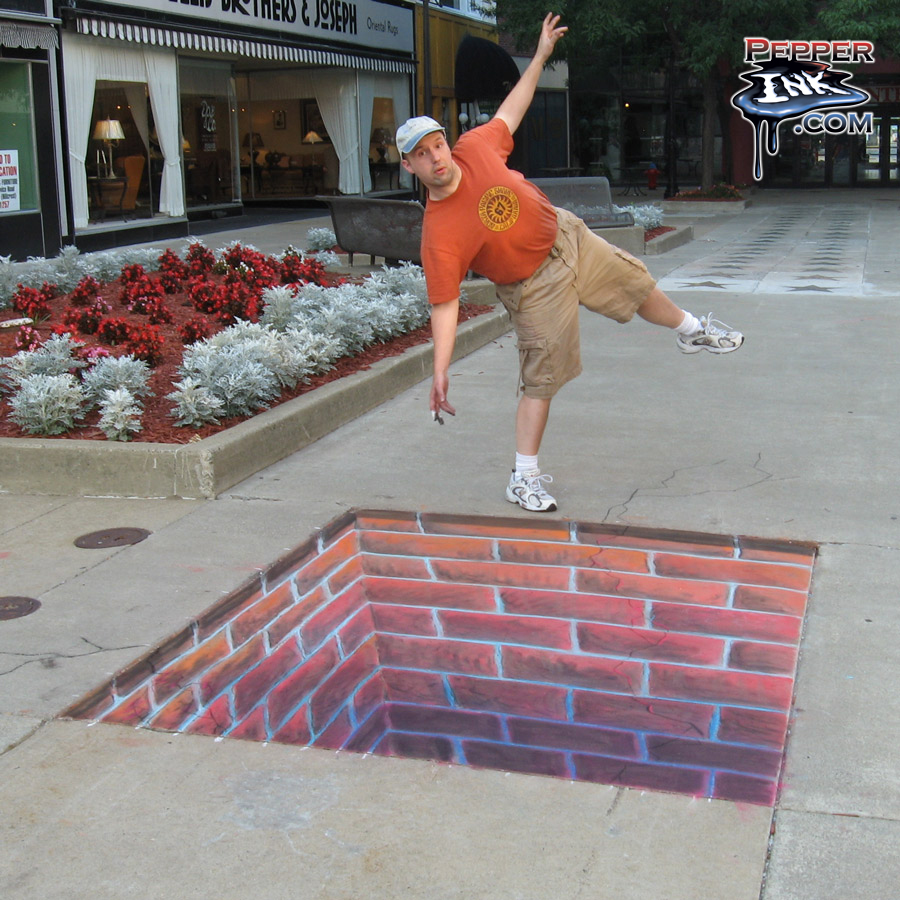
\includegraphics[scale=0.2]{q3/bricks.jpg}
        \subcaption{Original Image}
    \end{subfigure}
    \begin{subfigure}{.3\textwidth}
        \centering
        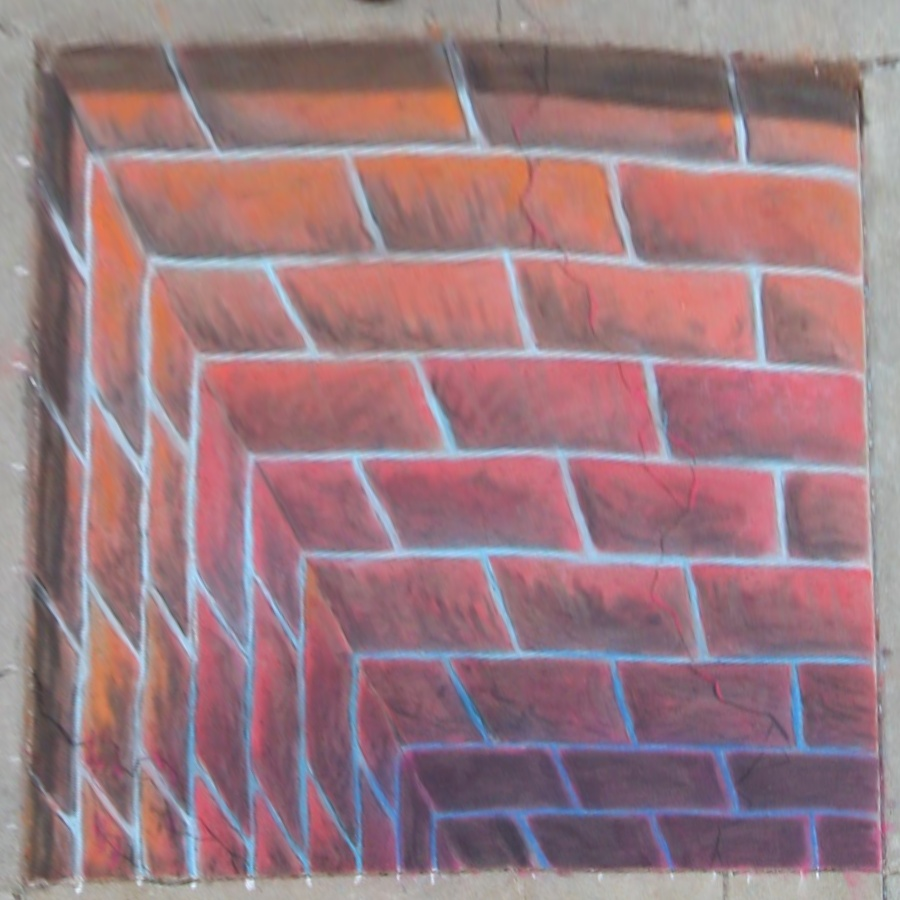
\includegraphics[scale=0.2]{q3/output.jpg}
        \subcaption{Perspective of 3D Art from above}  
        \label{fig 1}
    \end{subfigure}
\end{figure}
\subsection{Interpretation}
Given the source co-ordinates of the trapezium which are:
\newline{}
\texttt{[[344,499],[30,721],[847,531],[789,824]]}
\newline{}
and the destination co-ordinates of the square region we want to transform it into:
\newline{}
\texttt{[[0, 0], [0, 900], [900, 0], [900, 900]]}
When I applied the homography, the trapezium image is warped to fit into the square (as the tile covered by
 the artwork is square).

% https://tikz.net/zoom/
\end{document}

